\section{Evidence Lower Bound}

If we treat ${\phi}$ and ${\theta}$ as two optimization variables, we need an objective function (Loss function) to optimize these two parameters. The Loss function we use here is called Evidence Lower Bound (ELBO).

\subsection*{Definition (Evidence Lower Bound):}
\begin{equation}
\text{ELBO}(x) = \mathbb{E}_{q_\phi(z|x)} \left[ \log \frac{p(x, z)}{q_\phi(z|x)} \right].
\end{equation}

As mentioned earlier, \(p(x)\) is the marginal probability of the observation variable \(x\), calculated as:
\[
p(x) = \int p(x, z) \, dz = \int p(x \mid z) p(z) \, dz.
\]

\begin{itemize}
    \item We need to optimize this probability to motivate the model to achieve the best data distribution, thereby simulating and understanding the data. However, calculating this integral is very complicated due to the large space of \(z\) and the lack of a closed-form solution for \(p(x \mid z)\) and \(p(z)\).
    \item To address this, we build the relationship between \(p(x)\) and \(\text{ELBO}(x)\). We suggest the following theorem:
\end{itemize}

\subsection*{Theorem 1.1. Decomposition of Log-Likelihood:}
The log-likelihood \(\log p(x)\) can be decomposed as:
\[
\log p(x) = \mathbb{E}_{q_\phi(z|x)} \left[ \log \frac{p(x, z)}{q_\phi(z|x)} \right] + D_{\mathrm{KL}}(q_\phi(z|x) \| p(z|x)).
\]

\subsection*{Proof:}
Using \(q_\phi(z|x)\) as a proxy for \(p(x)\), we have:
\[
\log p(x) = \log p(x) \times \underbrace{\int q_\phi(z|x) dz}_{=1}.
\]

This implies:
\[
\log p(x) = \mathbb{E}_{q_\phi(z|x)} [\log p(x)].
\]

We define the Kullback-Leibler Divergence ~\cite{shlens2014kl} between two continuous distributions as:
\[
D_{\text{KL}}(P \,\|\, Q) = \int_{-\infty}^\infty p(x) \log \left( \frac{p(x)}{q(x)} \right) \, dx = \mathbb{E}_{p(x)} \left[\log \frac{p(x)}{q(x)} \right].
\]

\begin{figure}[H]
    \centering
    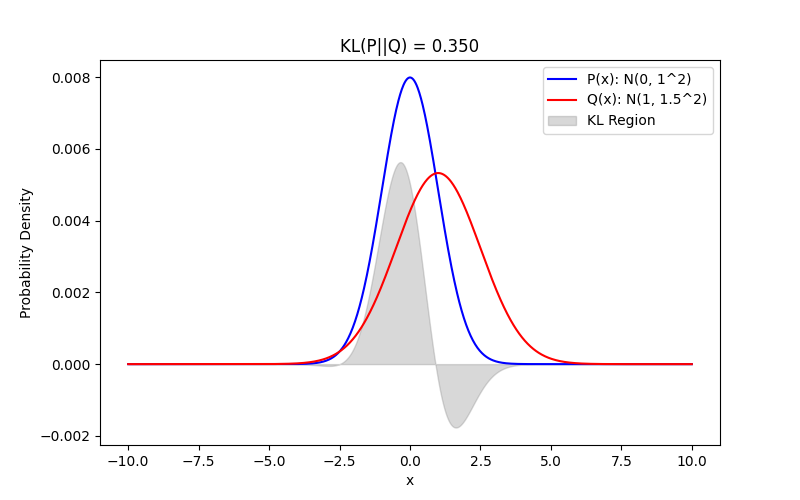
\includegraphics[width=1\linewidth]{sec/KL.png}
    \caption{Kullback-Leibler Divergence}
\end{figure}

Using Bayes' theorem (\(p(x, z) = p(z|x)p(x)\)) ~\cite{dosovitskiy2021imageworth16x16words}:
\[
\mathbb{E}_{q_\phi(z|x)}[\log p(x)] = \mathbb{E}_{q_\phi(z|x)} \left[\log \frac{p(x, z)}{p(z|x)}\right].
\]

Rewriting:
\begin{align}
\mathbb{E}_{q_\phi(z|x)} [\log p(x)] &= \mathbb{E}_{q_\phi(z|x)} 
\Big[ \log \frac{p(x, z)}{q_\phi(z|x)} \Big] \nonumber \\
&\quad + \mathbb{E}_{q_\phi(z|x)} 
\Big[ \log \frac{q_\phi(z|x)}{p(z|x)} \Big].
\end{align}


This simplifies to:
\[
\log p(x) = \text{ELBO}(x) + D_{\mathrm{KL}}(q_\phi(z|x) \| p(z|x)).
\]

\subsection*{Theorem 1.2. ELBO Decomposition:}
The ELBO can be expressed as:
\begin{equation}
\text{ELBO}(x) = \mathbb{E}_{q_\phi(z|x)} 
\big[\log p_\theta(x|z)\big] 
- D_{\text{KL}}(q_\phi(z|x) \| p(z)).
\end{equation}

\subsection*{Proof:}
Breaking the ELBO into two terms:
\begin{align*}
\text{ELBO}(x) &\overset{\text{def}}{=} \mathbb{E}_{q_\phi(z|x)} \big[ \log \frac{p(x, z)}{q_\phi(z|x)} \big] \\
&= \mathbb{E}_{q_\phi(z|x)} \big[ \log \frac{p(x|z)p(z)}{q_\phi(z|x)} \big] \\
&= \mathbb{E}_{q_\phi(z|x)} \big[ \log p(x|z) \big] + \mathbb{E}_{q_\phi(z|x)} \big[ \log \frac{p(z)}{q_\phi(z|x)} \big] \\
&= \mathbb{E}_{q_\phi(z|x)} \big[ \log p_\theta(x|z) \big] - D_{\text{KL}} \big( q_\phi(z|x) \| p(z) \big).
\end{align*}

\subsection*{ELBO Terms:}
\begin{itemize}
    \item \textbf{Reconstruction:} The first term, \(\mathbb{E}_{q_\phi(z|x)} [\log p_\theta(x|z)]\), measures the decoder's ability to reconstruct \(x\) from \(z\). This term is maximized when the decoder is accurate.
    \item \textbf{Prior Matching:} The second term, \(D_{\text{KL}}(q_\phi(z|x) \| p(z))\), regularizes \(q_\phi(z|x)\) to align with the prior \(p(z)\), typically \(\mathcal{N}(0, I)\).
\end{itemize}
